\subsection{Overview}

\subsubsection{Introduction}

\subsubsection{What's in the box}

\begin{figure}[htbp]
\centering
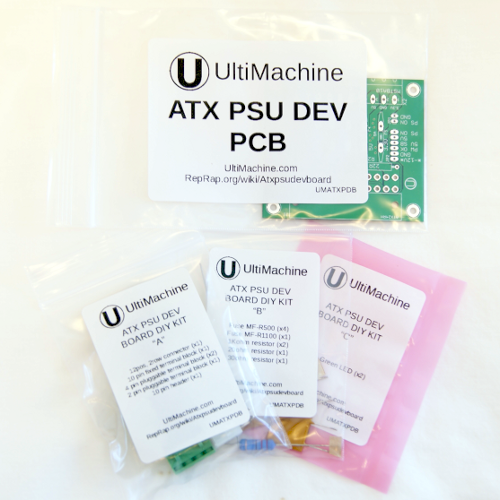
\includegraphics{./png/ATX_PSU_Dev_DIYkit.png}
\caption{Bag Layout}
\end{figure}

\subsection{Assembly}

\subsubsection{Preparation}

\paragraph{Tools}

The following tools and materials are required to assemble the ATX PSU
Dev Board:

\begin{itemize}
\item
  Soldering Iron
\item
  Solder
\item
  Flush/diagonal cutters
\end{itemize}

Additional tools that might be helpful, but not required:

\begin{itemize}
\item
  Lead bender
\end{itemize}

\paragraph{Soldering}

If you do not have prior experience soldering, we recommend checking out
a few of the following websites for some tutorials.

\begin{itemize}
\item
  \url{http://mightyohm.com/files/soldercomic/FullSolderComic_EN.pdf}
\item
  \url{http://www.ladyada.net/media/common/soldering.pdf}
\item
  \url{http://store.curiousinventor.com/guides/How_to_Solder}
\item
  \url{http://www.sparkfun.com/tutorials/106}
\item
  \url{http://radiojove.gsfc.nasa.gov/telescope/soldering.htm}
\end{itemize}

\subsubsection{Assembly}

The components of this board will be inserted on the side with the
outlines

Begin by inserting the two 1k$\Omega$ resistors and the LEDs into the
board. The LEDs should have the longest lead in the hole facing the
resistor. If they are inserted incorrectly they will not work. Resistors
are not polarized components, so they can be inserted in orientation.
\textbackslash{}

Next flip over the board and solder the components in. \textbackslash{}

The fuses will be inserted next. They have a coating that slightly
descends down the leads. \textbackslash{}

In order to make a good connection the fuses should slightly hover over
the holes. This is so the coating on the leads does not interfere with
soldering. You want to bring the fuse above the board. You can do this
with RepRap filament or something else, such as a long screw. The
orientation of the fuses does not matter.

Next you will want to solder in the remaining resistors. Again,
orientation does not matter for resistors.

Now is a good opportunity to check that all connections were soldered
well. Ideally the solder should wick up the lead onto the other side of
the board. It should also have a nice tapered look. Add some flux and
reheat the joint to touch-up the connections if needed. \textbackslash{}

Next you will want to add the ATX connector. It has barbs on the housing
that should clip onto the circuit board.

\section{Usage}

\subsection{Source}
